\documentclass[]{article}

\usepackage{mathtools} % Loads amsmath
\usepackage{graphics}
\usepackage{amsmath}
\usepackage{amssymb}
\usepackage{latexsym}
\usepackage{amsfonts}
\usepackage{authblk}
\usepackage{xfrac}
\usepackage{graphicx}
%\usepackage[colorlinks=true,linkcolor=black, citecolor=blue, urlcolor=blue]{hyperref} % for hyperrefs
%\usepackage{cleveref}
%\usepackage[authoryear]{natbib}
\usepackage{gensymb}  % provides macro \degree which works in text and math
\usepackage{color}
%\usepackage{enumitem} 
\usepackage{bm}
\usepackage{multirow}
\usepackage{cite}
\usepackage{tikz}
\usetikzlibrary{arrows}

% for quotes
\usepackage [english]{babel}
\usepackage [autostyle, english = american]{csquotes}
\MakeOuterQuote{"}

% For merging cells 
\usepackage{array}
\usepackage{booktabs}
\setlength{\heavyrulewidth}{1.5pt}
\setlength{\abovetopsep}{4pt}


% etc
%

\newcommand{\eq}[1]{Eq.~(\ref{#1})}
\newcommand{\eqnolabel}[1]{(\ref{#1})}
\newcommand{\eqs}[1]{Eqs.~(\ref{#1})}
\newcommand{\eqsthru}[2]{Eqs.~(\ref{#1})--(\ref{#2})}
\newcommand{\eqsand}[2]{Eqs.~(\ref{#1}) and (\ref{#2})}
\newcommand{\tbl}[1]{Table~\ref{#1}}
\newcommand{\tblnolabel}[1]{\ref{#1}}
\newcommand{\tbls}[1]{Tables~\ref{#1}}
\newcommand{\tblsthru}[2]{Tables~\ref{#1}--\ref{#2}}
\newcommand{\tblsand}[2]{Tables~\ref{#1} and \ref{#2}}
\newcommand{\fig}[1]{Fig.~\ref{#1}}
\newcommand{\fignolabel}[1]{\ref{#1}}
\newcommand{\figs}[1]{Figs.~\ref{#1}}
\newcommand{\figsthru}[2]{Figs.~\ref{#1}--\ref{#2}}
\newcommand{\figsand}[2]{Figs.~\ref{#1} and \ref{#2}}
\newcommand{\sxn}[1]{Section~\ref{#1}}

\newcommand{\revised}[1]{{\color{red}{#1}}}
\newcommand{\tsup}[1]{\textsuperscript{#1}}
\newcommand{\tsub}[1]{\textsubscript{#1}}

\newcommand{\erez}[1]{{\color{blue}{\textsuperscript{EREZ:}#1}}}
\newcommand{\roy}[1]{{\color{blue}{\textsuperscript{ROY:}#1}}}

\newcommand{\keff}{{\ensuremath{k_{\textrm{\scriptsize{eff}}}}}}
\newcommand{\beff}{\ensuremath{\beta_{\textrm{eff}}}}
\newcommand{\rr}{\ensuremath{\bm{r}}}
\newcommand{\OO}{\ensuremath{\hat{\bm{\Omega}}}}
\newcommand{\bnabla}{\ensuremath{\bm{\nabla}}}
\newcommand{\rE}{\ensuremath{(\rr,E)}}

\newcommand{\ftr}{\ensuremath{\phi_{\textrm{\scriptsize{tr}}}}}
\newcommand{\jtr}{\ensuremath{\bm{J}_{\textrm{\scriptsize{tr}}}}}
\newcommand{\jtrr}{\ensuremath{J_{\textrm{\scriptsize{tr}}}}}
%\newcommand{\mcL}{\mathcal{L}}
\newcommand{\mcL}{\tau}
\newcommand{\pl}[1]{\ensuremath{P_l(#1)}}
\newcommand{\dx}{\ensuremath{\Delta x}}

\newcommand{\jp}{\ensuremath{\bm{J}^+}}
\newcommand{\jm}{\ensuremath{\bm{J}^-}}
\newcommand{\jpm}{\ensuremath{\bm{J}^\pm}}
\newcommand{\jD}{\ensuremath{\bm{J}^{\textrm{\scriptsize{D}}}}}


%opening
\title{pCMFD for RM}
\author{}

\begin{document}

\maketitle

\begin{abstract}
Following Daniele Tomatis's notes. 
\end{abstract}

\section{Theoretical background}

The partial currents are defined according to (Duderstadt 1979):
\begin{equation}
\label{eq:partial-current}
\jpm (x) \approx \frac{\phi(x)}{4} \pm \frac{\jD(x)}{2} \,\, ,
\end{equation}
%where
%\begin{equation}
%\label{eq:diff-current}
%\bm{J} (x) = \jp(x) - \jm(x) \,\, .
%\end{equation}
Adding the partial currents (surface) correction factors
\begin{equation}
\label{eq:PCCF}
\jpm _{i+1/2} = \frac{1}{4}\phi_{i+1/2}
\pm \frac{1}{2} \jD _{i+1/2} \pm \frac{1}{2} \delta \jpm _{i+1/2} \,\, ,
\end{equation}
where
\begin{eqnarray}
\label{eq:jdiff}
\jD _{i+1/2} &=& - 2 D_{i+1/2} \frac{\phi_{i+1} - \phi_i}{\Delta_{i+1}+\Delta_i} \\
D_{i+1/2} &\equiv& \frac{\Delta_i D_i + \Delta_{i+1} D_{i+1}}{\Delta_i + \Delta_{i+1}} \\
\phi_{i+1/2} &\equiv& \frac{\Delta_i \phi_i + \Delta_{i+1} \phi_{i+1}}{\Delta_i + \Delta_{i+1}} \,\, .
\end{eqnarray}
Substituting
\begin{eqnarray}
\label{eq:CCF-sub}
\frac{1}{2} \delta \jp _{i+1/2} &\equiv& -\delta D^+ _{i+1/2} \phi_i \\
\frac{1}{2} \delta \jm _{i+1/2} &\equiv& -\delta D^- _{i+1/2} \phi_{i+1}\,\, ,
\end{eqnarray}
yields for CCFs
\begin{eqnarray}
\label{eq:par4}
\jp _{i+1/2} &=& \frac{1}{4}\phi_{i+1/2}
+ \frac{1}{2}\jD _{i+1/2} - \delta D^+ _{i+1/2} \phi_i \\
\jm _{i+1/2} &=& \frac{1}{4}\phi_{i+1/2}
- \frac{1}{2}\jD _{i+1/2} + \delta D^- _{i+1/2} \phi_{i+1} \,\, .
\end{eqnarray}
Recall that $\jpm$ are calculated using the integral expression. 
%
Solving for CCFs
\begin{eqnarray}
\label{eq:ccfsss1}
\delta D^+ _{i+1/2} &=& \frac{\frac{1}{4}\phi_{i+1/2}
	+ \frac{1}{2}\jD _{i+1/2} - \jp _{i+1/2}}{\phi_i} \\
\label{eq:ccfsss2}
\delta D^- _{i+1/2} &=& \frac{-\frac{1}{4}\phi_{i+1/2}
	+ \frac{1}{2}\jD _{i+1/2} + \jm _{i+1/2}}{\phi_{i+1}} \,\, .
\end{eqnarray}

In case the diffusion current is accurate, the CCFs should vanish and \eqsthru{eq:ccfsss1}{eq:ccfsss2} reduces back to \eq{eq:partial-current}, as expected, which imply for the total (accurate) current 
\begin{equation}
\bm{J} _{i+1/2} = \jp _{i+1/2} - \jm _{i+1/2} = \jD _{i+1/2} \,\, .
\end{equation} 
  

\begin{figure}[htbp]
	\centering
	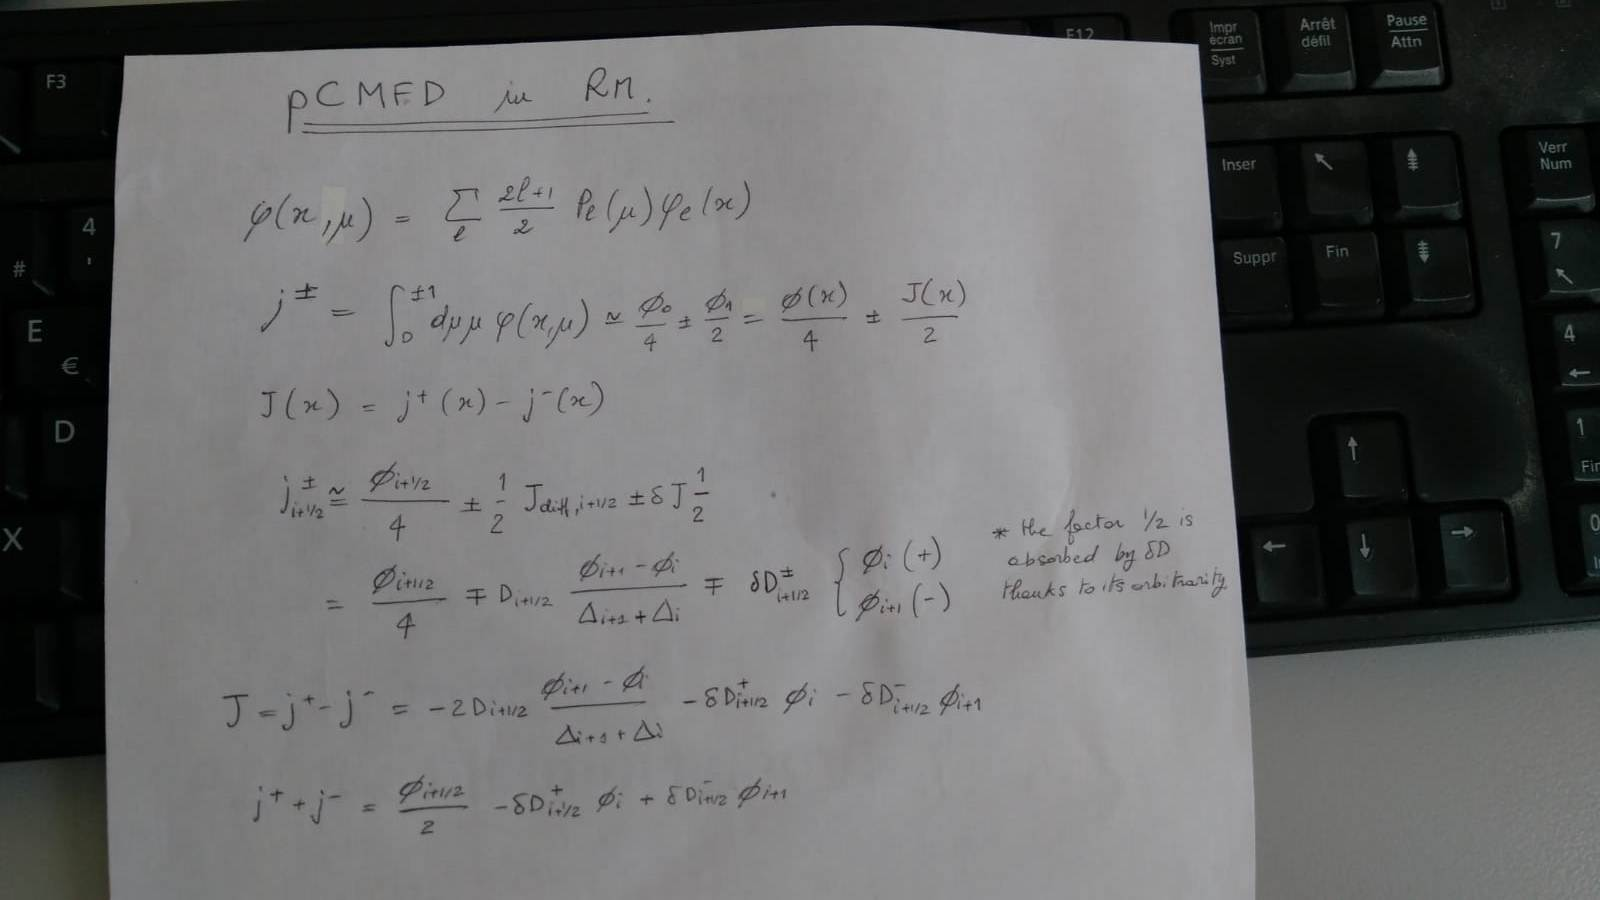
\includegraphics[width=.8\linewidth]{pCMFD-RM.png}
	\caption{Tomatis's notes.}
	\label{fig:Tnotes}
\end{figure}


\section{Numerical implementation}


 
\end{document}
